\documentclass[11pt,a4paper]{article}
\usepackage{od}
\usepackage[utf8]{inputenc}
\usepackage[russian]{babel}
\usepackage{tikz}
\usetikzlibrary{shapes.misc}
\usetikzlibrary{arrows.meta}

\pagestyle{headings}
\title{Кубок ТРИЗ-Саммита – 2019/2020}

\author{Трансформация текста в \LaTeX: Hans-Gert Gr\"abe, Leipzig}
\date{November 6, 2019}

\newcommand{\video}{Ролики должны быть короткие (от 2-х до 5 минут). Должны
  быть указаны все авторы этого сюжета: автор сценария, оператор, монтажер,
  актеры и т.д.

Данная работа направлена на формирование методического материала для обучения
ТРИЗ.

На сайте ТРИЗ
Саммита\footnote{\url{http://triz-summit.ru/ru/contest/competition/video/},\\
  \url{https://www.youtube.com/channel/UCjMNOjboWRBQA72DJvaC7ew/featured}}
опубликованы видеоролики, представленные на прошлый Кубок ТРИЗ Саммита.}

\newcommand{\credentials}{В подготовке заданий Кубка ТРИЗ Саммита-2018/2019
  принимали участие Рубин М.С., Рубина Н.В., номинация «фантазирование»
  подготовлена П.Р. Амнуэлем.}

\newcommand{\melies}{\begin{minipage}{.6\textwidth}
  \paragraph{1.}
  Основателем жанра научно-фантастический фильм является французский
  кинематографист Жорж Мельес. Каждый из более 500 короткометражных фильмов,
  созданных Мельесом, отличает неповторимый «режиссерский почерк». В фильме
  «Визит к обломкам крейсера «Мэн» (1897-1898) в эпизоде «водолазы за работой»
  надо было показать четкое изображение людей, работающих под водой, и такое
  же четкое изображение обломков крейсера. Фотографии под водой в это время
  уже делали, но они были скорее экзотикой не достаточно хорошее качество даже
  в очень прозрачной воде. Посмотрите, например, на одну из первых фотографий
  под водой, сделанную в 1893 году во Франции (согласитесь, качество не
  достаточное для эпизода фильма). Как же удалось снять эпизод под водой в
  хорошем качестве?
\end{minipage}\hfill
\begin{minipage}{.35\textwidth}
  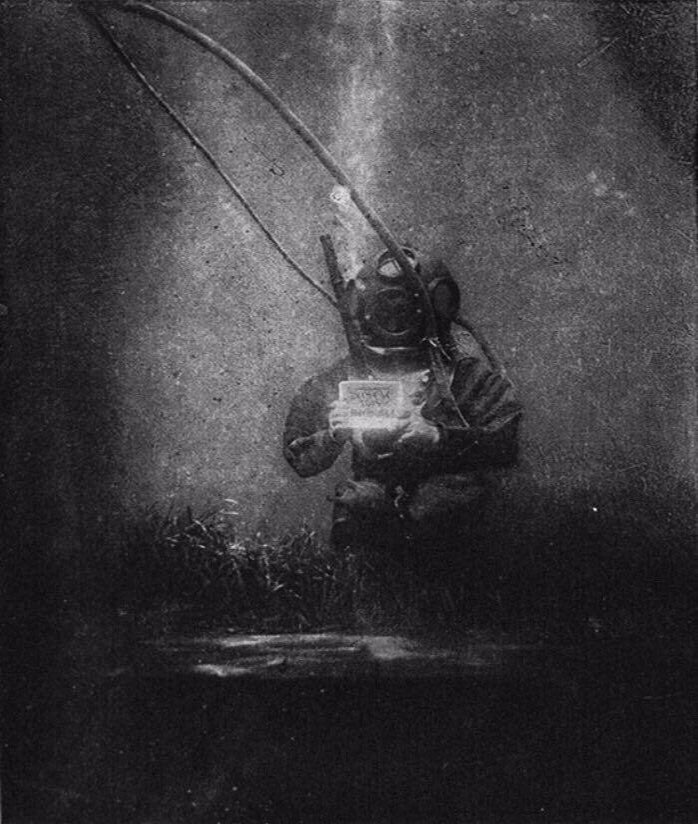
\includegraphics[width=\textwidth]{Bild-1.jpg}
\end{minipage}
\medskip

Фильм Ж. Мельеса «В царстве фей» с похожим эффектом можно посмотреть по
ссылке: \url{https://www.youtube.com/watch?v=paM_BPyRT1o&t=542s}

Удивительно, но такой же спецэффект использовал в фильме-сказке «Садко»
Александр Птушко в 1952 году в сценах на морском дне у Морского царя.

Какие еще спецэффекты применяются в кино, для решения каких задач? Какие
противоречия при этом возникают, какими приемами они разрешаются?
}

\newcommand{\hollywood}{\paragraph{2.}
В истории создания крупнейшего киноконцерна в мире – Голливуда – есть эпизоды,
связанные не с художественным творчеством, не с изобретением новых технических
средств для создания кино, а с чисто юридической проблемой. К началу XX века
человеком, владевшим основными патентами на киноаппаратуру в Америке, оказался
Томас Эдисон (тот самый изобретатель лампы накаливания). Однако большинство
кинематографистов того времени были основными собственниками независимых
кинокомпаний. Кроме того, все они работали на аппаратуре, которую сами
совершенствовали и приспосабливали к реализации придуманных ими идей
фильмов. По этим причинам они не считали необходимым выплачивать Эдисону
проценты за использование его патентов. 18 декабря 1908 года Эдисон объявил о
создании Motion Picture Patents Company (MPPC), которая вошла в историю кино,
как Трест Эдисона. В Компанию вступили несколько кинокомпаний, но большинство
предпочли остаться Независимыми. День 24 декабря 1908 года, когда вступила в
силу юрисдикция Треста, стал известен в истории американского кинематографа
как «черное Рождество». По правилам, введенным Эдисоном, Независимые
кинокомпании должны были выплачивать Тресту огромные суммы за право снимать и
демонстрировать кино. В Нью-Йорке под предлогом нарушения патентных прав
полиция закрыла 500 из 800 кинотеатров. Какое решение приняли Независимые
кинокомпании, чтобы не зависеть от Треста Эдисона?

Знаете ли вы примеры коммерческих, маркетинговых решений, которые
способствовали или тормозили развитие кино?
}

\newcommand{\kinogenres}{
\paragraph{1.}
Какие жанры кино вы знаете? Постройте хронологию появления различных жанров
кино. Выделите закономерности появления различных жанров в кино, какие события
в истории повлияли на появление и развитие различных жанров в кинематографе?
Выявите в развитии жанров кино Линии развития, закономерности, известные в
ТРИЗ? Какие жанры кино вам больше нравятся, почему?

\paragraph{2.}
В истории кино есть люди, чьи достижения и вклад в развитие кино очень
значительны, а имена забыты. Соберите информацию о биографиях этих
кинематографистов. Какие задачи они решали, какие приемы использовали? Как вы
думаете, какие Качества Творческой Личности помогли им достичь своих целей?
Часто решив конкретную задачу, человек останавливается на достигнутом, и не
может сделать больше ничего нового. Удивительно, но компания братьев Люмьер,
вошедших в историю, как создатели кинематографа, прекратила выпуск фильмов в
1900 году, всего через 5 лет после первого коммерческого показа фильмов 28
декабря 1895 года – дня рождения кино. Как вы думаете, что может помешать
человеку достигнуть значимых результатов в творчестве?
}

\newcommand{\kinotools}{\paragraph{1.}
Выберите несколько приемов, которые используются режиссерами, операторами,
звукооператорами, сценаристами (монтаж, паузы, спецэффекты, ускоренная или
замедленная съемка и т.д.) для получения каких-либо эффектов в кино.
Используйте эти приемы в своих роликах. Подробно раскройте ваш замысел в
описании к ролику. Можно ли усилить эти эффекты с помощью методов ТРИЗ?

\paragraph{2.}
Видеоролики по истории фотографии, кино и изобретениях, которые были сделаны в
этой области.
}

\begin{document}
\maketitle

Международная Общественная Организация «Саммит разработчиков ТРИЗ» объявляет о
проведении конкурса по Теории Решения Изобретательских Задач (ТРИЗ) для
школьников и студентов «Кубок ТРИЗ Саммита-2020». В конкурсе могут принять
участие учащиеся и студенты, изучающие ТРИЗ, а также преподаватели ТРИЗ.
Итоги конкурса будут подводиться по возрастным категориям: 8--10 лет; 11--14
лет; 15--17 лет; студенты; преподаватели.

Победители международного конкурса получают Дипломы, сертификаты участников и
памятные призы.  Конкурс продолжается до 22 марта 2020 года. Все материалы
принимаются в электронном виде. Адрес для переписки и отправки конкурсных
работ: \url{TDS-2015@yandex.ru}.

Это короткая версия информационного письма No 1. Точный текст можно найти на
страницах проекта
OpenDiscovery\footnote{\url{https://github.com/wumm-project/OpenDiscovery/tree/master/TRIZ-Cup/2020}}. 

\credentials
\vfill
\tableofcontents
\vfill
\clearpage
\section{Категория 8-10 лет}

\subsection*{Номинация «Изобретательство»}

\paragraph{1.}
При создании рисованного мультфильма необходимо разрешить несколько
противоречий:
\begin{itemize}
\item рисунков, составляющих мультфильм, должно быть как можно больше, чтобы
  изображение было плавным, без скачков, и их должно быть как можно меньше,
  чтобы сократить время создания мультфильма;
\item рисунки, составляющие мультфильм, должны быть с наибольшим количеством
  деталей, чтобы персонажи были эмоциональными, и должны быть с наименьшим
  количеством деталей, чтобы ускорить создание мультфильма;
\item камера, фиксирующая отдельные рисунки, должна быть неподвижной, чтобы
  изображение было четким и захватывало постепенно изменяющие положение
  объекты, и должна быть подвижной, чтобы захватывать разные ракурсы и объем
  пространства, окружающего объект.
\end{itemize}
Как разрешались эти противоречия в разных техниках создания мультфильмов?

\paragraph{2.}
Г.С. Альтшуллер в книге «Найти идею» предложил метод создания сюжетов для
мультфильма (или сказки), который можно назвать «Сказки с противоречиями».
Алгоритм создания такой сказки (сюжета для мультфильма) следующий:

\begin{enumerate}
\item Выбрать персонаж или объект сказочного сюжета.
\item Кратко представить себе окружение персонажа.
\item Применить прием фантазирования (увеличить, уменьшить, наоборот, оживить,
  бином фантазии и др.). Сформулировать сказочную \textsc{идею}.
\item Сформулироать анти-идею и противоречие. Построить сюжет на основе
  решения этого противоречия.
\item Ввести ограничение или создать новое противоречие в сюжете используя
  п. 3. Решения протиоречия - развитие сюжета.
\item Получается очень динамичный сюжет.
\end{enumerate}

Придумайте сюжет для мультфильма, используя этот алгоритм.

\subsection*{Номинация «Фантазирование»}

\paragraph{1.}
В 1974 году американский фантаст Джеймс Типри написал рассказ «Девушка,
которую подключили». В рассказе есть такой эпизод: фильм проецируют с помощью
лазеров на облака над городом, и все жители, глядя вверх, могут смотреть
кино. Сейчас это уже почти не фантастика – лазерные шоу на облаках стали
популярны. Однако это все-таки не фильмы. Придумайте новый, фантастический
способ демонстрации фильмов.

\paragraph{2.}
Советский фантаст Николай Василенко в рассказе «Кривое зеркало» (1977 год)
описал фантастическое зеркало: когда человек в него смотрится, то видит не
отражение, а небольшой фильм, в котором сущность глядящего в зеркало человека
предстает в образе какого-либо животного. Придумайте фантастический рассказ,
основанный на этой идее, но измените идею с помощью одного из приемов
фантазирования.

\subsection*{Номинация «Инструменты ТРИЗ»}

\paragraph{1.}
Из каких элементов состоит Мультстанок? Как они связаны между собой? Какие
функции выполняет каждый элемент? Из каких материалов можно изготовить
персонажей для мультфильма? Придумайте свой персонаж для мультфильма и
небольшую историю о нем.

\paragraph{2.}
Соберите картотеку примеров использования приемов фантазирования в
мультфильмах, фильмах-сказках. Проанализируйте картотеку. Какие приемы чаще
используются для создания типичных характеров или образов (как, например,
создается образ любопытного, озорного и отважного Буратино: длинный
(увеличенный) нос так и просится, чтобы «совать нос в чужие дела»; «ожившее»
полено «в воде не тонет, и в огне не горит»). Сравните, как в разных
мультфильмах (фильмах-сказках) создаются похожие образы (добрые и злые
волшебники, сильные богатыри, прекрасные принцессы, капризные принцессы и
т.д.). Какой у вас любимый мультфильм? Какие именно эпизоды в этом
мультфильме вам нравятся, используются ли в них приемы фантазирования?

\subsection*{Номинация «Исследования»}
Соберите картотеку мультфильмов об изобретателях (или ученых) и их
изобретениях (открытиях). Проанализируйте картотеку. Какие задачи решают в
этих мультфильмах их герои? Какие приемы использовались для решения задач? Как
применяются найденные решения (открытия) в жизни людей?

\subsection*{Номинация «Видеоролики по ТРИЗ»}
\begin{enumerate}\itemsep0pt
\item Выберите несколько приемов, которые используются режиссерами,
  операторами, звукооператорами, сценаристами (монтаж, паузы, спецэффекты,
  ускоренная или замедленная съемка и т.д.) для получения каких-либо эффектов
  в кино. Используйте эти приемы в своих роликах. Подробно раскройте ваш
  замысел в описании к ролику. Можно ли усилить эти эффекты с помощью методов
  ТРИЗ?
\item Видеоролики по истории фотографии, кино и изобретениях, которые были
  сделаны в этой области.
\end{enumerate}
\enlargethispage{5em}
\video

\clearpage
\section{Категория 11-14 лет}

\subsection*{Номинация «Изобретательство»}

\paragraph{1.}
В 1909 году американский кинематографист Дэвид Гриффит снял немой
короткометражный фильм (длительность 7 минут) «Уединенная
вилла»\footnote{\url{https://www.youtube.com/watch?time_continue=13&v=5RdbnyNYAv8}}. Это
остросюжетный фильм о попытке ограбления богатой уединенной виллы. Вероятно,
это самый первый фильм в жанре триллера (остросюжетный фильм, вызывающий у
зрителей напряжение и волнение). В фильме представлены три точки зрения:
\begin{itemize}
  \item семья, находящаяся в доме и спасающаяся от нападения;
  \item бандиты, нападающие на богатый дом;
  \item глава семьи и полицейские, появляющиеся в «последний момент».
\end{itemize}
У Гриффита была задача показать (за 7 минут) завязку этой истории,
проникновение в дом, страх хозяйки дома и трех ее дочерей, нападение и,
главное – спасение. До создания «Уединеннной виллы» кинофильмы содержали
сюжеты, охватывающие одно событие, и отражали последовательность действий
персонажей с хроникальной достоверностью (время в кино совпадало со временем
события в жизни). Как за короткое время фильма показать разные сюжетные линии
и усилить впечатление (напряжение) у зрителей? Какой кинематографический прием
впервые применил Д. Гриффит? Какие еще кинематографические приемы изобрел
Дэвид Гриффит и для создания каких эффектов они применялись? Выберите задачу
или несколько задач, которые решал Д. Гриффит и сделайте их разбор по
следующей схеме: сформулируйте противоречия, ИКР, перечислите ресурсы,
имеющиеся в задаче, приемы разрешения противоречий которые можно использовать
в этой задаче. Какие кинематографические приемы вы знаете, для решения каких
задач они применяются?

\paragraph{2.}
При создании рисованного мультфильма необходимо разрешить несколько противоречий:
\begin{itemize}
\item рисунков, составляющих мультфильм, должно быть как можно больше, чтобы
  изображение было плавным, без скачков, и рисунков должно быть как можно
  меньше, чтобы процесс создания мультфильма сократить во времени;
\item рисунки, составляющие мультфильм, должны быть с наибольшим количеством
  деталей, чтобы персонажи были эмоциональными, и должны быть с наименьшим
  количеством деталей, чтобы ускорить создание мультфильма;
\item камера, фиксирующая отдельные рисунки, должна быть неподвижной, чтобы
  изображение было четким и захватывало постепенно изменяющие положение
  объекты, и должна быть подвижной, чтобы захватывать разные ракурсы и объем
  пространства, окружающего объект.
\end{itemize}
Как разрешались эти противоречия в разных техниках создания мультфильмов?

\subsection*{Номинация «Фантазирование»}

\paragraph{1.}
Американский фантаст Томас Шерред в рассказе «Попытка» описал кинофильм,
снятый с помощью машины времени. Придумайте фантастический способ производства
кинофильмов. Как будут снимать фильмы в будущем?

\paragraph{2.}
В рассказе Павла Амнуэля «Летящий Орел» (1970 год) драматург, придумывая
пьесу, не пишет текст, как сейчас, а создает видеофильм, представляя себе,
будто пьеса уже поставлена. Ему не нужны актеры, он сам воображает персонажей,
их игру и поведение. Придумайте рассказ, основываясь на этой идее, но измените
ее с помощью какого-нибудь приема фантазирования.

\subsection*{Номинация «Инструменты ТРИЗ»}

Опишите технологический принцип действия кино. Из каких частей состоит КИНО?
Как эти части взаимодействуют между собой для получения кинематографического
эффекта? Какие эффекты (физические, химические, физиологические) используются
при создании и демонстрации кино? Как изменилось восприятие и мышление людей
за десятилетия существования кинематографа? Как вы думаете, какие эффекты
будут использоваться в кино в будущем?

\subsection*{Номинация «Исследования»}

\paragraph{1.}
Какие жанры кино вы знаете? Постройте хронологию появления различных жанров
кино. Можно ли на примере жанров в кино проиллюстрировать Линии развития
систем, известные в ТРИЗ (например, динамизация, моно-би-поли-свертывание,
переход в надсистему, переход на микроуровень). Какие жанры кино вам больше
нравятся, почему?

\paragraph{2.}
В 1927 году состоялась премьера фильма «Певец
джаза»\footnote{\url{https://my.mail.ru/mail/wikki0508/video/5622/29304.html}}
-- первый звуковой фильм в истории кинематографа. Современному зрителю уже
трудно представить фильм без слов и звуковых эффектов. Однако далеко не все
кинематографисты сразу приняли это революционное изменение. «Немота,
двухмерность и одноцветность фильма — не недостатки, а его «конструктивная
сущность». Киноискусство не нуждается в их преодолении, так как новые
выразительные средства только помешают дальнейшему его усовершенствованию», --
так писал об особенностях искусства кино Ю. Тынянов в 30-е годы. Попробуйте
доказать правоту противоположных точек зрения: выступите сначала на стороне
противников введения звука в кино, а затем на стороне сторонников этой
технологии.  Как вы думаете, какие новые эффекты звука появятся в кино в
будущем?

\subsection*{Номинация «Видеоролики по ТРИЗ»}
\kinotools

\video
\clearpage

\section{Категория 15-17 лет}

\subsection*{Номинация «Изобретательство»}

\melies

\hollywood

\subsection*{Номинация «Фантазирование»}

\paragraph{1.}
В романе американского фантаста Филипа Дика «Снятся ли андроидам электроовцы?»
описано устройство, позволяющее группе людей проникаться чувствами выбранного
человека, ощущать мир так, как ощущает он. Так можно снимать кино, и зрители
будут чувствовать все, что чувствовал актер во время съемок. Придумайте новую
фантастическую идею, изменив идею Дика с помощью «этажной схемы»
Г. С. Альтшуллера.

\paragraph{2.}
Александр Беляев в романе «Властелин мира» (1929 год) описал «мыслетеатр», в
котором актеры не играют на сцене, они лишь мысленно представляют свою игру, а
зритель эти мысли «ловит» и мысленно «видит» спектакль. Придумайте
фантастический рассказ о съемках такого «мыслефильма», изменив идею Беляева с
помощью одного из приемов фантазирования.

\subsection*{Номинация «Инструменты ТРИЗ»}

В развитии технических систем можно выделить несколько Линий развития,
например, «моно-би-поли-свертывание»; «динамизация»; «пустотности»; «переход
на микроуровень»; «личное – лично-коллективное – коллективное». Соберите
картотеку примеров, иллюстрирующих эти Линии развития в области кино или
фотографии. Учтите, что и кино и фотография – это и искусство, и технология
производства, и коммерческий продукт (кинотеатры, реклама, сопутствующий
сервис и т.д.).

\subsection*{Номинация «Исследования»}
\kinogenres

\subsection*{Номинация «Видеоролики по ТРИЗ»}
\kinotools

\video
\clearpage

\section{Категория студенты}

\subsection*{Номинация «Изобретательство»}

\melies

\hollywood

\subsection*{Номинация «Фантазирование»}

\paragraph{1.}
В фантастических рассказах японского писателя Кобо Абэ «Тоталоскоп» и
итальснского писателя Лино Алдани «Онирофильм» (оба рассказа опубликованы в
1965 году) описаны фильмы, снятые с полным эффектом присутствия и обратной
связью со зрителем. Измените эту идею с помощью приемов фантазирования,
использовав не один прием, а несколько. Опишите результат.

\paragraph{2.}
Американский фантаст Френк Херберт в космической эпопее «Дюна» (1965 год)
описал, как один из персонажей управляет поведением других людей с помощью
особых интонаций голоса. При этом человек, которым управляют, прекрасно это
понимает, но ничего поделать не может: он вынужден подчиняться. Придумайте
сюжет для приключенческого фильма будущего, взяв за основу идею Херберта, но
изменяя ее по мере развития сюжета с помощью приемов фантазирования.

\subsection*{Номинация «Инструменты ТРИЗ»}

Законы развития технических систем – основа ТРИЗ. Существуют несколько
возможных классификаций этих законов. Предлагаем вам одну из них.
\begin{center}
\newcommand{\law}[2]{\parbox{#1cm}{\small\centering #2}}
\tikz[>={Triangle[length=3pt 9, width=3pt 3]}] {
  
\node[draw] at (5,7) [rectangle]
(A1) {\law{3}{Закон повышения идеальности}};

\node[draw] at (0,6) [rectangle]
(A2) {\law{4}{Закон повышения полноты частей системы (Закон полноты выполнения принципа действия)}};

\node[draw] at (0,2) [rectangle]
(A3) {\law{4}{Закон повышения согласованности частей системы}};

\node[draw] at (0,4) [rectangle]
(A4) {\law{4}{Закон проводимости: энергии, потоков и др.)}};

\node[draw] at (5,5) [rectangle]
(A5) {\law{3}{Закон неравномерного развития частей системы}};

\node[draw] at (10,0) [rectangle]
(A6) {\law{4}{Тенденция развития ТС по S-образной кривой}};

\node[draw] at (0,0) [rectangle]
(A7) {\law{4}{Тенденция вытеснения человека из ТС}};

\node[draw] at (10,4) [rectangle]
(A8) {\law{4}{Закон повышения управляемости / вепольности}};

\node[draw] at (5,1) [rectangle]
(A9) {\law{3}{Закон повышения динамичности}};

\node[draw] at (5,3) [rectangle]
(A10) {\law{3}{Закон перехода в надсистему}};

\node[draw] at (10,6) [rectangle]
(A11) {\law{4}{Закон перехода с макроуровня на микроуровень}};

\node[draw] at (10,2) [rectangle]
(A12) {\law{4}{Тенденция развития за счет свертывания или развертывания ТС}};

\draw[->] (A1) -- (2.8,7) |- (A2) ;
\draw[->] (2.8,7) |- (A3);
\draw[->] (2.8,7) |- (A4);
\draw[->] (2.8,7) |- (A7);
\draw[->] (2.8,7) |- (A9);
\draw[->] (2.8,7) |- (A10);
\draw[->] (A2) -- (-2.7,6) |- (A7);
\draw[->] (A5) -- (7.2,5) |- (A9);
\draw[->] (7.2,5) |- (A10);
\draw[->] (7.2,5) |- (A6);
\draw[->] (A1) -- (7.5,7) |- (A8) ;
\draw[->] (7.5,7) |- (A11) ;
\draw[->] (7.5,7) |- (A12) ;
\draw[->] (A8) -- (12.5,4) |- (A12) ;
}
\end{center}
Проанализируйте этапы развития кинематографа, используя систему Законов
Развития Технических Систем. Как, учитывая выявленные вами тенденции в
развитии кинематографа, можно спрогнозировать дальнейшее развитие кино?

\subsection*{Номинация «Исследования»}
\kinogenres

\subsection*{Номинация «Видеоролики по ТРИЗ»}
\kinotools

\video

\end{document}
